\documentclass[../../main.tex]{subfiles}

% 

\begin{document}
\chapter{Registrácia a detekcia ionizujúceho žiarenia}

Ionizujúce žiarenie je okom neviditeľné, takže aby sme sa o jeho existencii vôbec mohli presvedčiť, je treba ho detekovať pomocou príslušných fyzikálnych metód a vhodnej prístrojovej techniky. Okrem \quotedblbase zviditeľnenia\textquotedblright ~nám detekcia umožňuje skúmať vlastnosti tohto žiarenia a využívať ho v množstve vedecko-technických, priemyslových a medicínskych aplikácií. Poskytuje nám kvantitatívne informácie o intenzite, energii, priestorovej distribúcii a príp. ďalších vlastnostiach žiarenia.

\section{Druhy detektorov ionizujúceho žiarenia}

Bola vyvinutá rada detektorov ionizujúceho žiarenia, ktoré (okrem spoločného základného javu, ktorým sú ionizačné účinky žiarenia) využívajú rôzne princípy a technické konštrukcie. Prístroje na detekciu ionizujúceho žiarenia sa niekedy označujú súhrnným názvom \textbf{rádiometre}. Fungujú buď samostatne, alebo sú súčasťou prístrojov na meranie niektorých veličín a monitorovanie určitých dejov pomocou radiačných metód.

Špeciálnym typom rádiometrov sú tzv. dozimetre. Sú to väčšinou jednoduché detekčné prístroje, ktoré sú cejchované v jednotkách radiačnej dávky (Gray, Sievert) či dávkového príkonu. Používajú sa pri radiačnom monitorovaní na posudzovanie účinku žiarenia predovšetkým na živé tkanivo.  

Detektory ionizujúceho žiarenia môžeme rozdeliť podľa troch kritérií: časový priebeh detekcie, fyzikálno-technický princíp detekcie a komplexnosť meranej radiačnej informácie.

Podľa časového priebehu detekcie rozoznávame dve základné skupiny detektorov:
\begin{itemize}
\item \textbf{Kontinuálne (online) detektory} - poskytujú priebežnú informáciu o okamžitej intenzite žiarenia či počte kvánt ionizujúceho žiarenia. Odozva takéhoto detektoru by mala byť úmerná okamžitej intenzite žiarenia. Ak detektor prestane byť ožarovaný, signál na jeho výstupe poklesne na nulu, či na hodnotu pozadia. Detektory tohto druhu sú takmer vždy elektronické.

\item \textbf{Kumulatívne (integrálne) detektory} - postupne zhromažďujú svoju rastúcu odozvu behom expozície. Táto odozva zostáva v detektore uchovaná aj po skončení expozície a môže sa vyhodnotiť dodatočne. Vyhodnotením sa získa údaj o celkovej hodnote ožiarenia za celú dobu, počas ktorej bol detektor vystavený ožiareniu.
\end{itemize}

Rôzne druhy detektorov poskytujú odozvu na interakciu častíc rôznymi, často veľmi odlišnými, spôsobmi. Líšia sa preto svojimi vlastnosťami a tým aj možnosťami a oblasťou svojho využitia. Podľa princípu detekcie rozoznávame tri skupiny detektorov:
\begin{itemize}
\item \textbf{Fotografické} - založené na fotochemických účinkoch žiarenia (filmové dozimetre, rtg filmy, jadrové emulzie), alebo využívajúce fotografické zobrazenie stôp častíc v určitom látkovom prostredí (hmlové a bublinkové komory).

\item \textbf{Materiálové} - využívajúce dlhodobejšej zmeny vlastností určitých vhodných látok (zloženie, objem, farba) pôsobením ionizujúceho žiarenia. Ťažké častice (predovšetkým $\alpha$) zanechávajú v materiály určité stopy, ktoré sa dajú zviditeľniť či detekovať. Vzhľadom k nízkej citlivosti sú použiteľné iba pre vysoké intenzity či dlhodobú kumulatívnu detekciu. Pri väčšine materiálových kumulatívnych detektorov sa stretávame s nepriaznivým javom zvaným \textit{fading} - slabnutím odozvy detektoru s časom, k čomu dochádza priebežne v období medzi ožiarením a vyhodnotením. V dôsledku fyzikálnych a chemických vplyvov v materiály detektoru dochádza k spontánnemu miznutiu latentného obrazu vo fotografických materiáloch, či ku spontánnej deexcitácii metastabilných elektrónových hladín termoluminiscenčných dozimetrov.

\item \textbf{Elektronické detektory} - v nich sa časť absorbovanej energie ionizačného žiarenia prevádza na elektrické prúdy či impulzy, ktoré sa zosilňujú a vyhodnocujú v elektronických aparatúrach. Vstupná časť detekčného prístroja je vlastný detektor - čidlo zariadenia, ktoré prevádza časť energie žiarenia na merateľnú elektrickú odozvu. Tá sa potom spracováva v elektronických obvodoch rádiometra a zobrazuje sa alebo zapisuje v registračnom zariadení. Medzi elektronické detektory patria plynové ionizačné komory, scintilačné detektory, polovodičové detektory, mikrokalorimetrické detektory, magnetické spektrometre.
\end{itemize}

Ionizujúce žiarenie, ktoré potrebujeme detekovať, sa často skladá z častíc a kvánt rôzneho druhu a energie, ktoré prichádzajú z rôznych smerov a miest v priestore, z rôznych rádioaktívnych, elektronických či kozmických zdrojov. Podľa komplexnosti meranej informácie môžeme meracie prístroje ionizujúceho žiarenia rozdeliť na 4 skupiny:
\begin{itemize}
\item \textbf{Detektory žiarenia} - prevádzajú obyčajnú registráciu interakcií častíc s detektorom, s príp. určením časového okamžiku interakcie. Udávajú iba intenzitu žiarenia, resp. počet kvánt žiarenia, bez informácie o druhu žiarenia a jeho energii. Tieto nespektrometrické detektory neposkytujú informácie o energii žiarenia a môžu byť použité iba na základnú detekciu častíc alebo fotónov. Medzi tieto najjednoduchšie detektory patria filmové a termoluminiscenčné dozimetre, ionizačné komory vrátane GM detektorov.

\item \textbf{Spektrometre ionizujúceho žiarenia} - merajú nielen intenzitu či počet kvánt žiarenia, ale aj energiu kvánt a príp. jeho ďalšie charakteristiky. Výsledkom je väčšinou energetické spektrum $N=N(E)$, zachytávajúce graficky závislosť početnosti $N$ na energii $E$. Spektrum teda vyjadruje energetické rozloženie kvánt študovaného žiarenia. Jedným z druhov spektrometrov sú tzv. kalorimetre - detekčné systémy, ktoré absorbujú všetku energiu častice a ich výstupná odozva je úmerná tejto energii. Používajú sa predovšetkým na analýzu vysokoenergetického žiarenia vznikajúceho pri interakciach rýchlych častíc. Tieto energetické častice nepredávajú v látke svoju energiu pri jednej či niekoľkých málo interakciách, ale vytvárajú kaskády sekundárnych častíc, ktoré sa môžu ďalej vetviť na ďalšie spŕšky, zasahujúce veľké objemy látky.

\item \textbf{Zobrazovacie detektory} - kamery, ktoré zobrazujú (vizuálne alebo elektronicky) priestorové rozloženie intenzity žiarenia. Najjednoduchším zobrazovacím detektorom je fotografický film. V rtg diagnostike sa tiež používala luminiscenčné tienidlá, ktoré boli neskôr doplnené zosilňovačmi obrazu a príp. elektronickým spracovávaním. Dnes sa používajú multidetektorové systémy priestorovo vhodne rozmiestnených detektorov, ktoré poskytujú informácie o miestach dopadu žiarenia, alebo o uhloch, z ktorých žiarenie prilieta. Príkladom sú scintilačné kamery.

\item \textbf{Dráhové detektory častíc} - merajú dráhy pohybu jednotlivých častíc v priestore, vrátane ich zakrivenia v magnetickom poli. Dosahuje sa to buď na základe materiálových efektov (fotochemické reakcie, kondenzácia kvapôčiek z pary alebo vznik bubliniek v prehriatej kvapaline) alebo elektronicky zložitými systémami veľkého množstva priestorovo rozmiestnených detektorov, polovodičových alebo ionizačných komôr - súhrnne nazývaných \textit{trackery}. Analýzou dráh častíc, či už priamych či rôzne zakrivených v magnetickom poli, alebo rozvetvujúcich sa dráh v dôsledku zrážok a interkacií, sa získavajú informácie o vlastnostiach elementárnych častíc, jadrových a časticových interakciách.
\end{itemize}

\section{Tienenie, kolimácia a filtrácia detekovaného žiarenia}

V mnohých prípadoch nestačí umiestniť samotný \quotedblbase holý\textquotedblright ~detektor požadovaného žiarenia do určitého miesta a registrovať prichádzajúce kvantá. Okrem vlastného analyzovaného žiarenia sa v mieste merania takmer vždy vyskytuje aj ďalšie nežiadúce a rušivé žiarenie. Je to jednak prírodné žiarenie (rádioaktivita prostredia, kozmické žiarenie), žiarenie z prípadných ďalších okolných zdrojov, niekedy aj nežiadúce zložky v samotnom meranom žiarení. Na elimináciu či obmedzenie týchto rušivých radiačných vplyvov sa detektor vybavuje ďalšími vhodnými mechanickými či elektronickými dielmi, čím sa zväzok či pole detekovaného žiarenia upraví v zásade tromi spôsobmi

\begin{itemize}
\item \textbf{Tienenie detektoru}

Na potlačenie nežiadúceho žiarenia z okolia je treba vlastný detektor obklopiť dostatočne silným obalom z látky dobre absorbujúcej žiarenie - umiestniť detektor do vhodného tienenia. Najčastejším  konštrukčným materiálom na tienenie $\gamma$ žiarenia je olovo, v špeciálnych prípadoch sa používa aj wolfrám a iné materiály. Niekedy používame aj čiastočné odtienenie primárneho detekovaného žiarenia - predovšetkým v prípade silného žiarenia, ktoré by zahltilo citlivý detektor.

V materiály tienenia dochádza k interakciám detekovaného žiarenia s atómami látky, čo môže viesť ku vzniku sekundárneho žiarenia. Okrem Comptonovského rozptylu, generujúceho žiarenie so spojitým spektrom, je to aj fotoefekt, doprevádzaný vznikom charakteristického r"ontgenového žiarenia s čiarovým spektrom. Na obr. \ref{em3:img:tienenie} vidíme vplyv rôznych typov tienenia scintilačného detektoru na tvar spektra meranej vzorky rádionuklidu $^{99m}$Tc, emitujúceho žiarenie gama s energiou 140 keV. Pri detektore bez tienenia (a) je pred fotopíkom celkom nevýrazné monotónne Comptonovské kontinuum. Pre meranie nízkych aktivít je nutné umiestniť detektor dovnútra masívneho oloveného tienenia (b). Vedľajším efektom tohto užitočného opatrenia je interakcia gama fotónov s atómami tienenia napr. fotoefektom, pri ktorom vzniká sekundárne charakteristické r"ontgenové žiarenie olova s energiou cca 70-80 keV, ktoré sa uplatňuje v spektre. Špeciálnym druhom tienenia sú kolimátory, používané ako primárny zobrazovací element v scintigrafii. Interakciou gama fotónov fotoefektom s olovenými prepážkami medzi otvormi kolimátoru vzniká taktiež charakteristické r"ontgenové žiarenie olova. Pokiaľ má kolimátor relatívne hrubé prepážky (cca 0,5 mm), je charakteristické žiarenie olova účinne absorbované a v spektre prejdeného žiarenia vidíme iba nevýrazný X-pík (c). Pri kolimátoroch LE UHR s drobnými otvormi a veľmi tenkými prepážkami dochádza k výraznému prežiarovaniu gama aj charakteristického r"ontgenového žiarenia olova, takže v spektre môže byť r"ontgenovský fotopík dokonca výraznejší, než primárny fotopík 140 keV.

\begin{figure}[h]
\centering
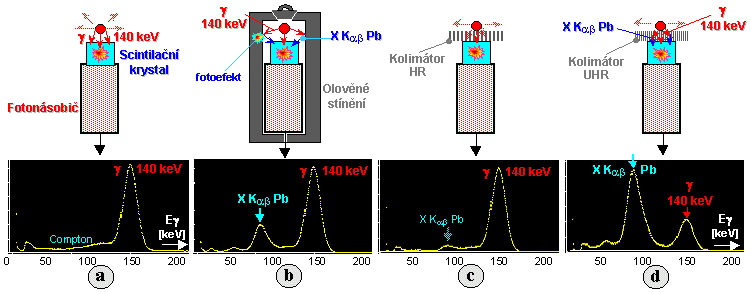
\includegraphics[width=\textwidth]{em3-tienenie.png}
\caption{Vplyv rôznej geometrie tienenia detektoru na scintilačné spektrum. a) Základné scintilačné spektrum vzorky $^{99m}$Tc nameranej detektorom bez tienenia. b) Spektrum namerané detektorom vnútri oloveného tienenia (7cm Pb). c) Spektrum namerané cez olovená scintigrafický kolimátor typu HR. d) Spektrum cez kolimátor UHR s drobnými otvormi.}
\label{em3:img:tienenie}
\end{figure}

\item \textbf{Kolimácia detekovaného žiarenia}

V prípade, že potrebujeme detekovať iba žiarenie prichádzajúce z určitého smeru, opatríme detektor kolimátorom - takým mechanickým a geometrickým usporiadaním materiálov absorbujúcich daný druh žiarenia, ktoré prepustí iba žiarenie prichádzajúce z určitých požadovaných smerov (uhlov), zatiaľ čo žiarenia z iných smerov absorbuje a neprepúšťa. Najjednoduchšie kolimátory majú tvar rôznych tubusov a clôn. Špeciálne zložité konfigurované zobrazovacie kolimátory s veľkým počtom otvorov hrajú kľúčovú úlohu v scintigrafii. Rôzne druhy špeciálne tvarovaných kolimátorov sa používajú v rádioterapii, najdôležitejší je mnoholamelový multi-leaf kolimátor MLC.

Okrem vyššie uvedenej priamočiarej \quotedblbase fyzickej\textquotedblright ~kolimácie žiarenia sa v niektorých špeciálnych detekčných systémoch používa aj iný spôsob smerovej selekcie žiarenia, tzv. elektronická kolimácia, bez použitia mechanického kolimátoru. Je založená na špecifickom chovaní kvánt ionizujúceho žiarenia v detekčnom systéme - šírení dvojíc (či viac) kvánt v určitých presne daných smeroch, ich koincidenčnú detekciu sústavou väčšieho počtu detektorov a následnej pozičnej a uhlovej rekonštrukcii smeru šírenia kvánt. Táto analýza umožňuje vyberať k ďalšiemu spracovaniu iba také kvantá žiarenia, ktoré majú požadovaný smer - prevádzať elektronickú kolimáciu a zobrazenie distribúcie žiarenia v danom poli. Metóda elektronickej kolimácie sa používa v pozitrónovej emisnej tomografii PET.


\item \textbf{Filtrácia detekovaného žiarenia}

Používa sa v špeciálnych prípadoch, kedy vlastné merané žiarenie obsahuje kvantá alebo častice rôznych druhov a energií, pričom potrebujeme merať iba jednu zo zložiek primárneho žiarenia a ostatných sa chceme zbaviť. 

Príkladom môže byť meranie rádionuklidovej čistoty preparátov v prípade, že daný základný rádionuklid emitujúci žiarenie $\gamma$ s nízkou energiou je kontaminovaný malou prímesou rádionuklidu vyžarujúceho vyššiu energiu. Pri priamom meraní by bol detektor zahltený základným žiarením nižšej energie, v ktorého záplave by sa riedko prichádzajúce vysokoenergetické fotóny strácali. V takomto prípade možno s výhodou použiť metódu filtrácie tieniacou absorpčnou vložkou: fľaštičku so skúmaným preparátom umiestnime do oloveného tienenia vhodnej hrúbky, ktoré takmer úplne pohltí intenzívne nízkoenergetické žiarenie, avšak prepustí značnú časť slabého, avšak vysokoenergetického $\gamma$ žiarenia kontaminantu.

\end{itemize}

Pri použití kolimácie a filtrácie si musíme byť vedomí toho, že určitá časť prichádzajúceho žiarenia nebude detekovaná, dochádza ku zníženiu detekčnej účinnosti. Pri kvantitatívnych meraniach je preto treba na túto okolnosť spraviť príslušnú korekciu, či ju zahrnúť do kalibrácie detekčného systému.

\end{document}